\chapter{Normal Operation}

To further our understanding of wind turbine operation and prepare a more detailed analysis, we need a fundamental intuition of how turbines behave under normal operating conditions. A single turbine will have three control parameters; yaw, pitch, and rotational speed. However, since yawing would never benefit a single turbine under normal wind conditions, this chapter will primarily investigate the relationship between pitch and rotational speed. We will also explore how dimensionless numbers compare with their associated quantities and how they are relevant in further analysis. 

\section{Setup}

Consider a turbine standing on a plane field with no significant obstacles in the near vicinity. As there is nothing obvious to disturb the flow, we might assume that the air behaves relatively linearly within our theoretical test volume, and we may therefore approximate this with a simple uniform flow. Note that this might not give a perfect representation of the loads in a more practical situation, but it should be sufficient to explain how the turbine wants to behave for a given flow velocity. Since calculations for such a simplified example are very cheap computationally, we will look into a wide range of velocities. More specifically, the simulation starts with a speed of $5 \; m/s$ and steadily increases up to $25 \; m/s$ and back again, in steps of  $1 \; m/s$. These sudden increases between each step will create small fluctuations in the data, which we will have to compensate for. A simple way to do this is to calculate each quantity for all data points with a velocity within a range of the current step. We can then take the average of these values, giving us a good estimation, assuming that the fluctuations are equally distributed around each step. To illustrate the given range and steps, an exaggerated velocity curve is shown in figure \ref{fig:fluctuationillu}.

\begin{figure}[H]
    \centering
    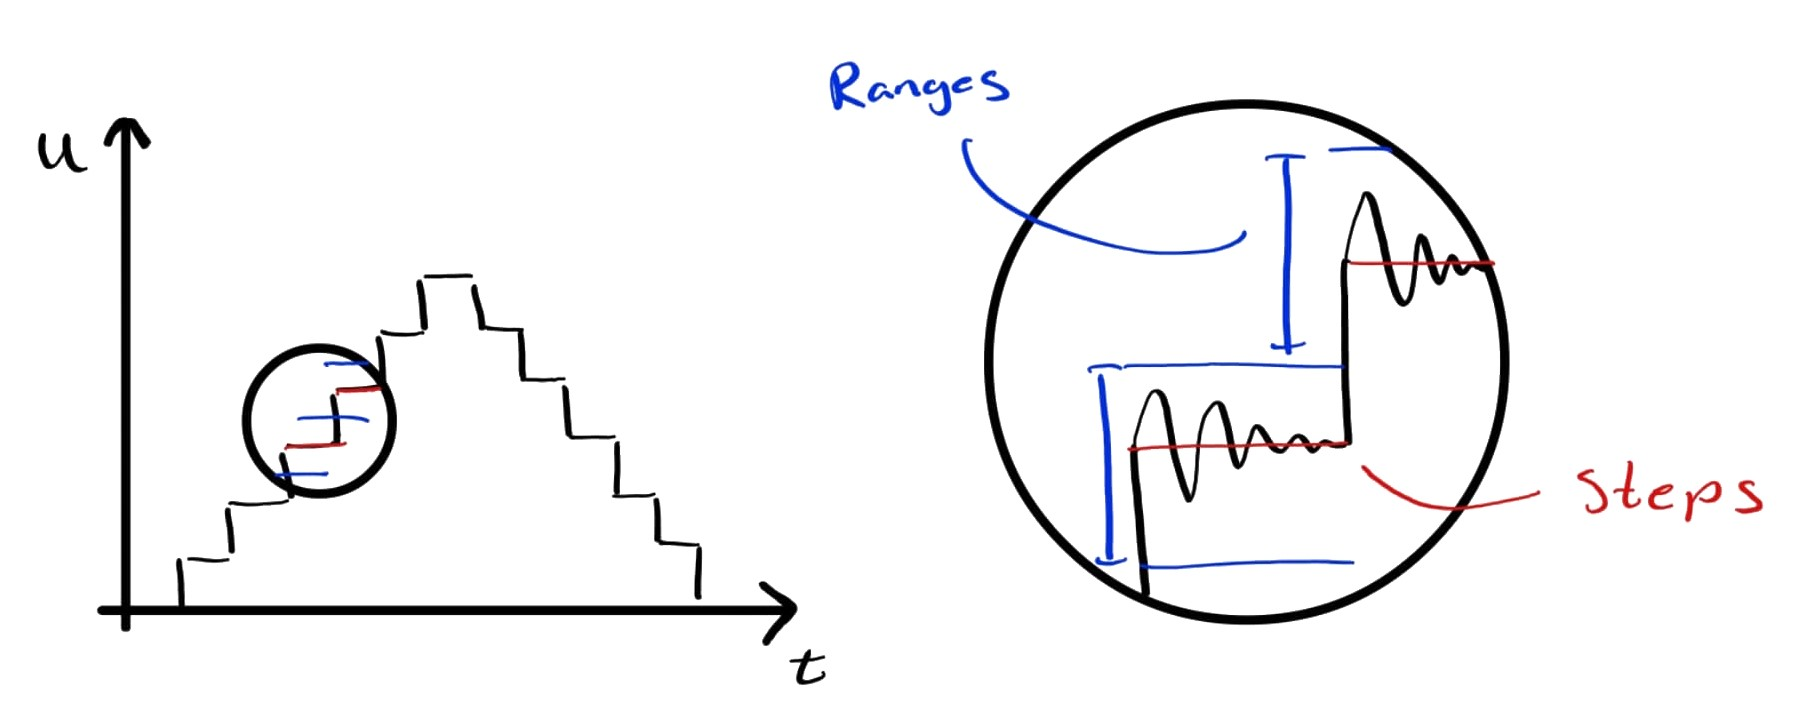
\includegraphics[scale=0.24]{Illustrations/fluctuation_illu.jpg}
    \caption{Illustration of exaggerated fluctuations on velocity curve for uniform inflow}
    \label{fig:fluctuationillu}
\end{figure}

%%%%%%%%%%%%%%%%%%%%%%%%%%%%%%%%%%%%%%%%%%%%%%%%%%%%%%%%%%%%%%%%
\section{Pitch and rotational speed}

As a starting point, we would like the wind turbine to produce as much electricity as possible. However, when increasing the velocity above a certain threshold, we might encounter physical limitations regarding how fast the turbine can rotate and what force it can withstand without collapsing. In practice, this means that we have a maximum rated power output and that we have to purposely take less energy from the air by pitching if proceeding this limit. Since power and rotational speed are almost proportional, we will compare rotational speed $\Omega$ and pitch $\theta$ as a function of flow velocity $U$, which is illustrated in figure \ref{fig:rotpitch}.

\begin{figure}[H]
    \centering
    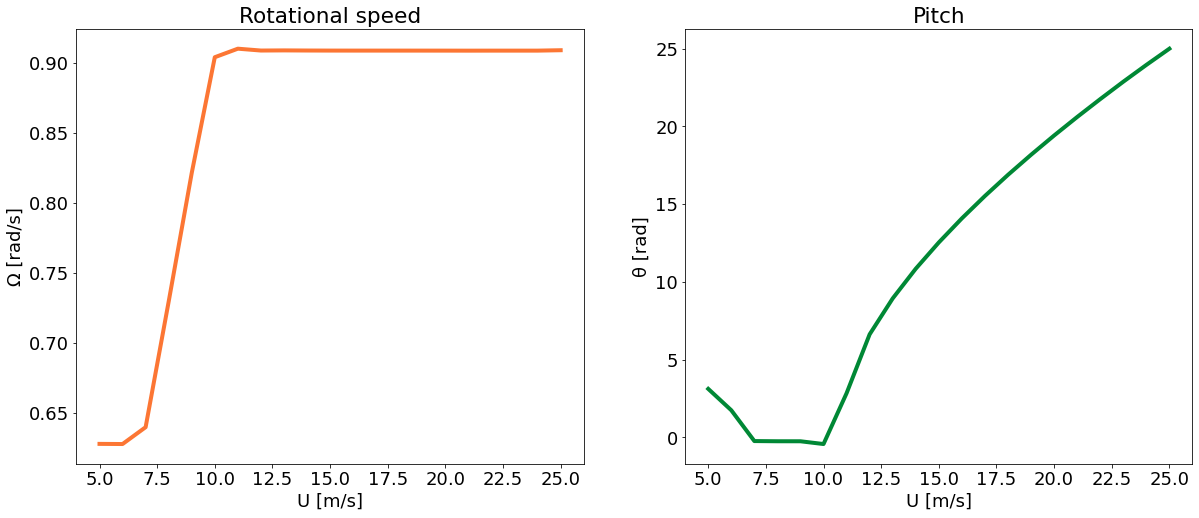
\includegraphics[scale=0.3]{Illustrations/rotpitch.png}
    \caption{Rotational speed and Pitch as a function of velocity}
    \label{fig:rotpitch}
\end{figure}

As we might expect, it is seen that the turbine extracts as much energy as possible from the air for low wind speeds. In this region, the rated power/rotational speed has yet to be reached, and it does not make sense to pitch the blades. However, at approximately $10 \; m/s$, the rotational speed reaches its maximum and stays constant for the remaining velocities. For this range, the pitching is determined automatically to match the rating and turns out to have a slightly curved relation between angle and incoming velocity. Knowing how the power and thrust behaves is also quite interesting if we want an understanding of normal operation. The plot of these is seen in figure \ref{fig:powerthrust}.

\begin{figure}[H]
    \centering
    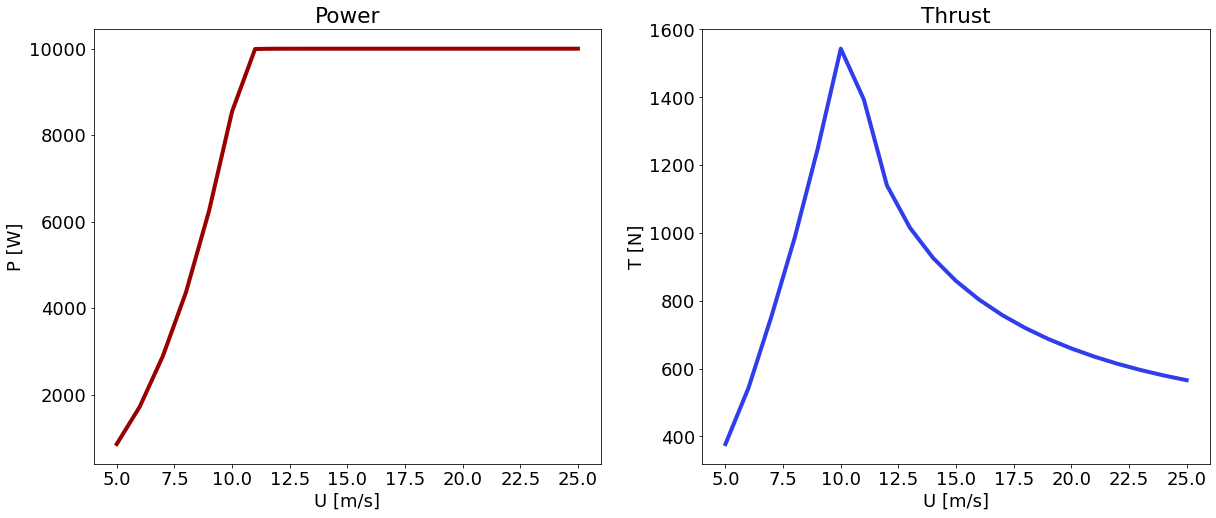
\includegraphics[scale=0.3]{Illustrations/powerthrust.png}
    \caption{Power and Thrust as a function of velocity}
    \label{fig:powerthrust}
\end{figure}

The graphs are very predictable, considering the previously mentioned arguments regarding the rated power limitations. Here we see that similar to the rotational speed the power increases almost linearly up to the rated value and will afterwards stay constant at $10 \: MW$. The trust has a very similar profile until that $10 \frac{m}{s}$ mark where the pitching starts. In actuality, power and thrust can be proven to follow a third and second-order polynomial, respectively. However, regarding them as linear is adequate for a basic understanding of the operation \cite{dimentionlesspower}. After that, it will steadily decrease as the blades turn into the wind and encounter less resistance. 

%%%%%%%%%%%%%%%%%%%%%%%%%%%%%%%%%%%%%%%%%%%%%%%%%%%%%%%%%%%
\section{Dimensionless analysis}

One might also be interested in how the power production and thrust compare to the wind condition in terms of potential energy and momentum. We can investigate such by plotting the ratio between Power/thrust and their reference value as a dimensionless number. The ratios can be expressed as

\begin{equation}
    C_P = \frac{P}{\frac{1}{2} \rho A U^3}, \quad C_T = \frac{T}{\frac{1}{2} \rho A U^2} 
\end{equation}

Plotting as a function of $U$ yields the graphs displayed in figure \ref{fig:powerthrust}

\begin{figure}[H]
    \centering
    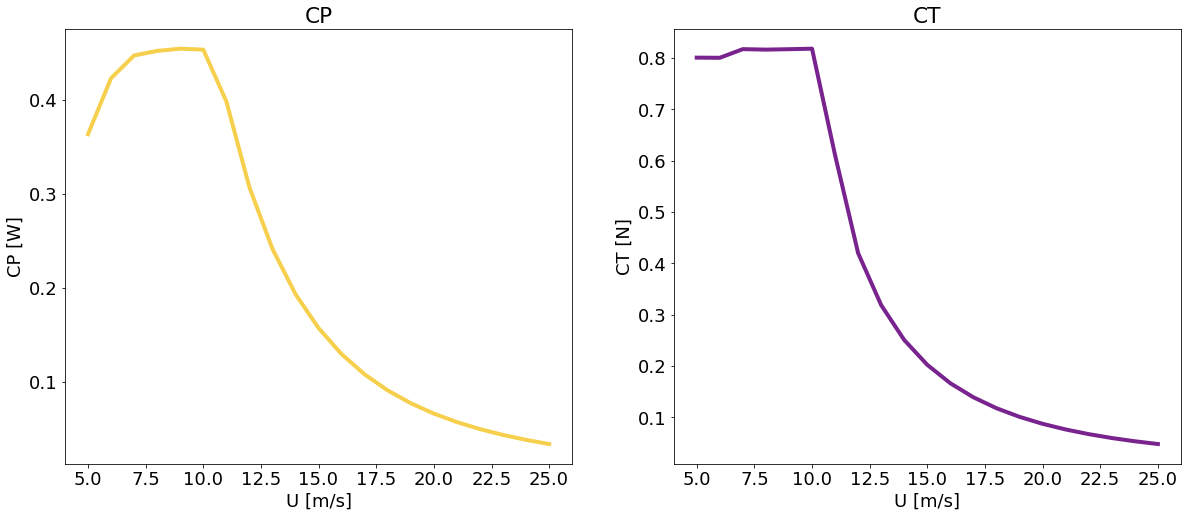
\includegraphics[scale=0.3]{Illustrations/CPCTsweep.png}
    \caption{$C_P$ and $C_T$ as a function of velocity}
    \label{fig:powerthrust}
\end{figure}

Starting with the power, we can see that for very low wind speeds, the turbine struggles to extract as much energy as it wants. After that, there is a small range from about $6 \; m/s$ to  $10 \; m/s$, where the value is constant at roughly $C_P=0.46$. Interestingly, this is not the period of highest energy production but rather a practical limit of how much of the energy potential we can extract. The value is about what we expect for a modern turbine and is a substantial percentage of the theoretical max at just over $59\%$ \cite{betzlimit}. Lastly, our ratio decreases rapidly as the faster velocities contain a lot of energy that we cannot extract with the given turbine. For the thrust, we can primarily use the same argument. However, what is notable is that the value for low speeds is much higher than $C_P$. This means, in practice, that the turbine experience much greater loads relative to the power produced than it would for higher wind speeds. This is very much in conformity with the thrust graph and means that though we will not produce more energy at higher velocities, it is still beneficial due to the lower loads resulting in a longer lifespan. 